\documentclass[t, 12pt, numbers, fleqn, handout]{beamer}
%\documentclass[t,12pt,numbers,fleqn]{beamer}
%\documentclass[ignorenonframetext]{beamer}

\newif\ifquestions
%\questionstrue
\questionsfalse

\usepackage{pgfpages} 
\usepackage{hyperref}
\hypersetup{colorlinks=true,
    linkcolor=blue,
    citecolor=blue,
    filecolor=blue,
    urlcolor=blue,
    unicode=false}
\urlstyle{same}

\usepackage{booktabs}
\usepackage{multirow}

\bibliographystyle{plain}

%\usetheme{Iimenau}

\useoutertheme{split} %so the footline can be seen, without needing pgfpages

%\pgfpagesuselayout{resize to}[letterpaper,border shrink=5mm,landscape]  %if this is uncommented, the hyperref links do not work

\mode<presentation>{}

\input{../def-beamer}

\newcommand{\topic}{14 Module Interface Specification (MIS)}

%Title page information for 1D04 lectures slides

% Define year specific parameters - used in title page and footer

\newcommand{\season}{Fall} %use to switch between Winter and Fall
\newcommand{\instructor}{Dr.~Spencer Smith} %use to switch instructor
\newcommand{\instructSmall}{Dr.~Smith}
\newcommand{\yr}{2019}
\newcommand{\courseCode}{CAS 741, CES 741}
\newcommand{\courseTitle}{Development of Scientific Computing Software}

%\setbeamerfont{structure}{series=\bfseries}
%\usefonttheme[stillsansseriftext,stillsansserifmath]{serif}
\setbeamertemplate{navigation symbols}{} 
\setbeamertemplate{itemize item}[ball]

\title{
  {\normalsize \bf 
    \borange{\courseCode~(\courseTitle)\\ \season~\yr}}\\[2ex]
  {\Large \bf \topic}}

\author[Smith]{\instructor}

\institute{
  Faculty of Engineering,
  McMaster University}

\date{
\today
%January 2011\\
\bc
  \includegraphics[scale = 0.2, keepaspectratio]
  {../mcmaster-logo-full-color.jpg}
\ec
}

\renewcommand{\borange}[1] %orange is too hard to read
{
   \bred{#1}
}

\begin{document}

\input{../footline}

%%%%%%%%%%%%%%%%%%%%%%%%%%%%%%%%%%%%%%%%%%%%%%%%%%%%%%

\begin{frame}
\frametitle{Module Interface Specification (MIS)}

\bi
\item Administrative details
\item Questions?
\item Finish previous day slides
\item Module guide example
\item Integration testing
\item Mathematical review (\cite{HoffmanAndStrooper1995} and separate slides)
\begin{itemize}
\item Multiple assignment statement
\item Conditional rules
\item etc.
\end{itemize}
\item MIS overview
\item Modules with external interaction
\item Abstract objects
\item Abstract data types
\item Generic MIS
\item Inheritance
\ei
\end{frame}

%%%%%%%%%%%%%%%%%%%%%%%%%%%%%%%%%%%%%%%%%%%%%%%%%%%%%%

\begin{frame}
\frametitle{Administrative Details}

\bi
\item VnV GitHub issues for colleagues
\bi
\item Assigned 1 colleague (see \texttt{Repos.xlsx} in repo)
\item Provide at least 5 issues on their VnV Plan
\item Grading as before
\item Due by Friday, Oct 26, 11:59 pm
\item If you have an extension past today, please let your partner know
\item If your partner has an extension, you have three days after their deadline
 \ei
  
%\item For MG presentation, we'll try to use my laptop only
\item Template for MG in repo

\ei

\end{frame}

%%%%%%%%%%%%%%%%%%%%%%%%%%%%%%%%%%%%%%%%%%%%%%%%%%%%%%

\begin{frame}
\frametitle{Administrative Details: Deadlines}
~\newline
\begin{tabular}{l l l}
\textbf{MG Present} & Week 08 & Week of Oct 29\\
\textbf{MG} & Week 09 & Nov 5\\
MIS Present & Week 10 & Week of Nov 12\\
MIS & Week 11 & Nov 19\\
Unit VnV or Impl.\ Present & Week 12 & Week of Nov 26\\
Unit VnV Plan & Week 13 & Dec 3\\
Final Doc & Week 14 & Dec 10\\
\end {tabular}

\end{frame}

%%%%%%%%%%%%%%%%%%%%%%%%%%%%%%%%%%%%%%%%%%%%%%%%%%%%%%

\begin{frame}
\frametitle{Administrative Details: Presentation Schedule}

\bi
\item MG Present
\bi
\item \textbf{Wednesday: Karol, Malavika, Robert, Hanane}
\item \textbf{Friday: Brooks, Vajiheh, Olu, Jennifer}
\ei
\item MIS Present
\bi
\item Wednesday: Malavika, Robert
\item Friday: Hanane,  Jennifer
\ei
\item Unit VnV Plan or Impl.\ Present
\bi
\item Wednesday: Brooks, Vajiheh
\item Friday: Olu, Karol
\ei
\ei

\end{frame}

%%%%%%%%%%%%%%%%%%%%%%%%%%%%%%%%%%%%%%%%%%%%%%%%%%%%%%

\begin{frame}
\frametitle{Questions?}
\begin{itemize}
\item Questions about Module Guide and the presentation?
\end{itemize}
\end{frame}

%%%%%%%%%%%%%%%%%%%%%%%%%%%%%%%%%%%%%%%%%%%%%%%%%%%%%%

\begin{frame}
\frametitle{Finish Previous Day's Discussion}
\begin{itemize}
\item Static Definition of Uses Relation
\item Module Guide
\item MG Template
\item MG Verification
\item OO versus modular
\end{itemize}
\end{frame}

%%%%%%%%%%%%%%%%%%%%%%%%%%%%%%%%%%%%%%%%%%%%%%%%%%%%%%

\begin{frame}
\frametitle{Solar Water Heating System Example}

\bi
\item \href{https://github.com/smiths/swhs}{https://github.com/smiths/swhs}
\item Solve ODEs for temperature of water and PCM
\item Solve for energy in water and PCM
\item Generate plots
\ei

\begin{figure}
{
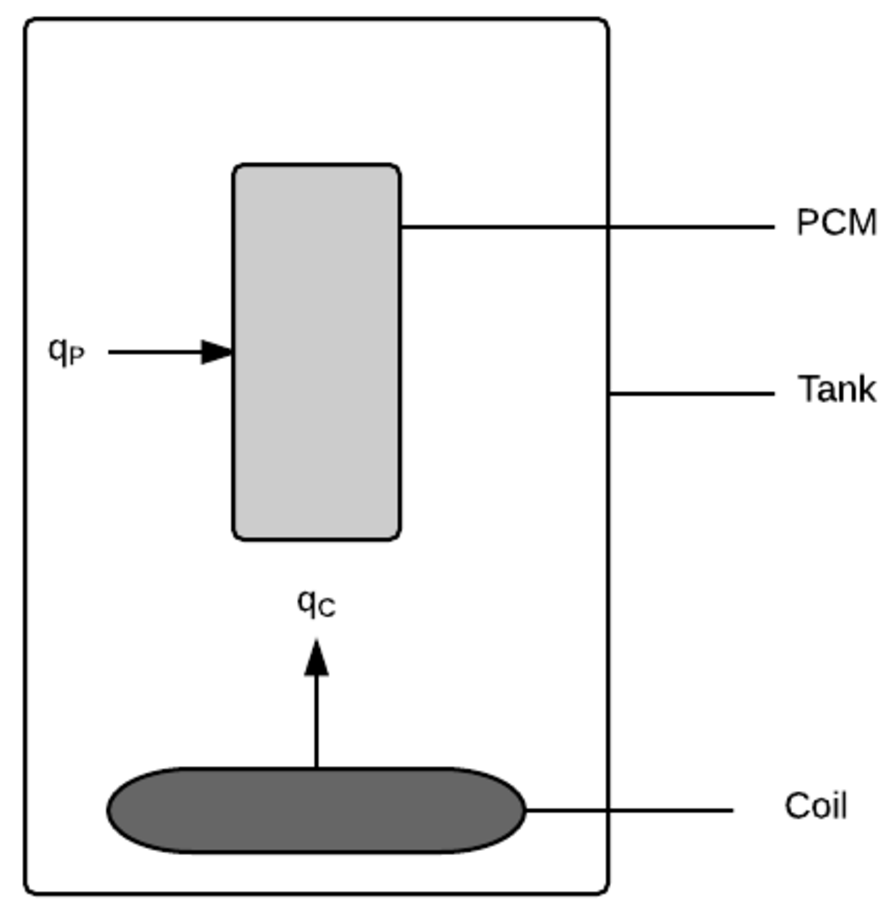
\includegraphics[width=0.5\textwidth]{../Figures/Tank.pdf}
}
\end{figure}

\end{frame}

%%%%%%%%%%%%%%%%%%%%%%%%%%%%%%%%%%%%%%%%%%%%%%%%%%%%%%

\begin{frame}
\frametitle{Anticipated Changes?}

\structure{What are some anticipated changes?}\\
~\newline
Hint: the software follows the Input $\rightarrow$ Calculate $\rightarrow$
Output design pattern

\end{frame}

%%%%%%%%%%%%%%%%%%%%%%%%%%%%%%%%%%%%%%%%%%%%%%%%%%%%%%

\begin{frame}
\frametitle{Anticipated Changes}

\bi
\item The specific hardware on which the software is to run
\item The format of the initial input data
\item The format of the input parameters
\item The constraints on the input parameters
\item The format of the output data
\item The constraints on the output results
\item How the governing ODEs are defined using the input parameters
\item How the energy equations are defined using the input parameters
\item How the overall control of the calculations is orchestrated
\item The implementation of the sequence data structure
\item The algorithm used for the ODE solver
\item The implementation of plotting data
\ei

\end{frame}

%%%%%%%%%%%%%%%%%%%%%%%%%%%%%%%%%%%%%%%%%%%%%%%%%%%%%%

\begin{frame}
\frametitle{Module Hierarchy by Secrets}
\begin{table}[h!]
\centering
\begin{tabular}{p{0.3\textwidth} p{0.6\textwidth}}
\toprule
\textbf{Level 1} & \textbf{Level 2}\\
\midrule

{Hardware-Hiding Module} & ~ \\
\midrule

\multirow{6}{0.3\textwidth}{Behaviour-Hiding Module} & Input Parameters Module\\
& Output Format Module\\
& Temperature ODEs Module\\
& Energy Equations Module\\ 
& Control Module\\
& Specification Parameters\\
\midrule

\multirow{3}{0.3\textwidth}{Software Decision Module} & {Sequence Data Structure Module}\\
& ODE Solver Module\\
& Plotting Module\\
\bottomrule

\end{tabular}
\caption{Module Hierarchy}
\label{TblMH}
\end{table}
\end{frame}

%%%%%%%%%%%%%%%%%%%%%%%%%%%%%%%%%%%%%%%%%%%%%%%%%%%%%%

\begin{frame}
\frametitle{Example Modules from SWHS}

\textbf{Hardware Hiding Modules}

\begin{description}
\item[Secrets:] The data structure and algorithm used to implement the virtual
  hardware.
\item[Services:] Serves as a virtual hardware used by the rest of the
  system. This module provides the interface between the hardware and the
  software. So, the system can use it to display outputs or to accept inputs.
\item[Implemented By:] OS
\end{description}

\end{frame}

%%%%%%%%%%%%%%%%%%%%%%%%%%%%%%%%%%%%%%%%%%%%%%%%%%%%%%

\begin{frame}
\frametitle{Example Modules from SWHS}

\textbf{Input Parameters Module}

\begin{description}
\item[Secrets:] The data structure for input parameters, how the
values are input and how the values are verified.  The load and verify secrets
are isolated to their own access programs (like submodules). %    This, combined
% with the fact that all of the services are invoked together, suggests that the
% one module one secret rule can be relaxed here.
\item[Services:] Gets input from user (including material properties, processing
  conditions, and numerical parameters), stores input and verifies that the
  input parameters comply with physical and software constraints. Throws an
  error if a parameter violates a physical constraint. Throws a warning if a
  parameter violates a software constraint.  % Stored parameters can be read
  % individually, but write access is only to redefine the entire set of inputs.
\item[Implemented By:] SWHS
\end{description}

\end{frame}

%%%%%%%%%%%%%%%%%%%%%%%%%%%%%%%%%%%%%%%%%%%%%%%%%%%%%%

\begin{frame}
\frametitle{Example Modules from SWHS}

\textbf{ODE Solver Module}

\begin{description}
\item[Secrets:] The algorithm to solve a system of first order ODEs initial
  value problem from a given starting time until the given event function shows
  termination.
\item[Services:] Solves an ODE using the governing equation, initial
  conditions, event function and numerical parameters.
\item[Implemented By:] Matlab
\end{description}

\end{frame}

%%%%%%%%%%%%%%%%%%%%%%%%%%%%%%%%%%%%%%%%%%%%%%%%%%%%%%

\begin{frame}[plain, fragile]

\frametitle{SWHS Uses Hierarchy (approximately)}

\begin{center}
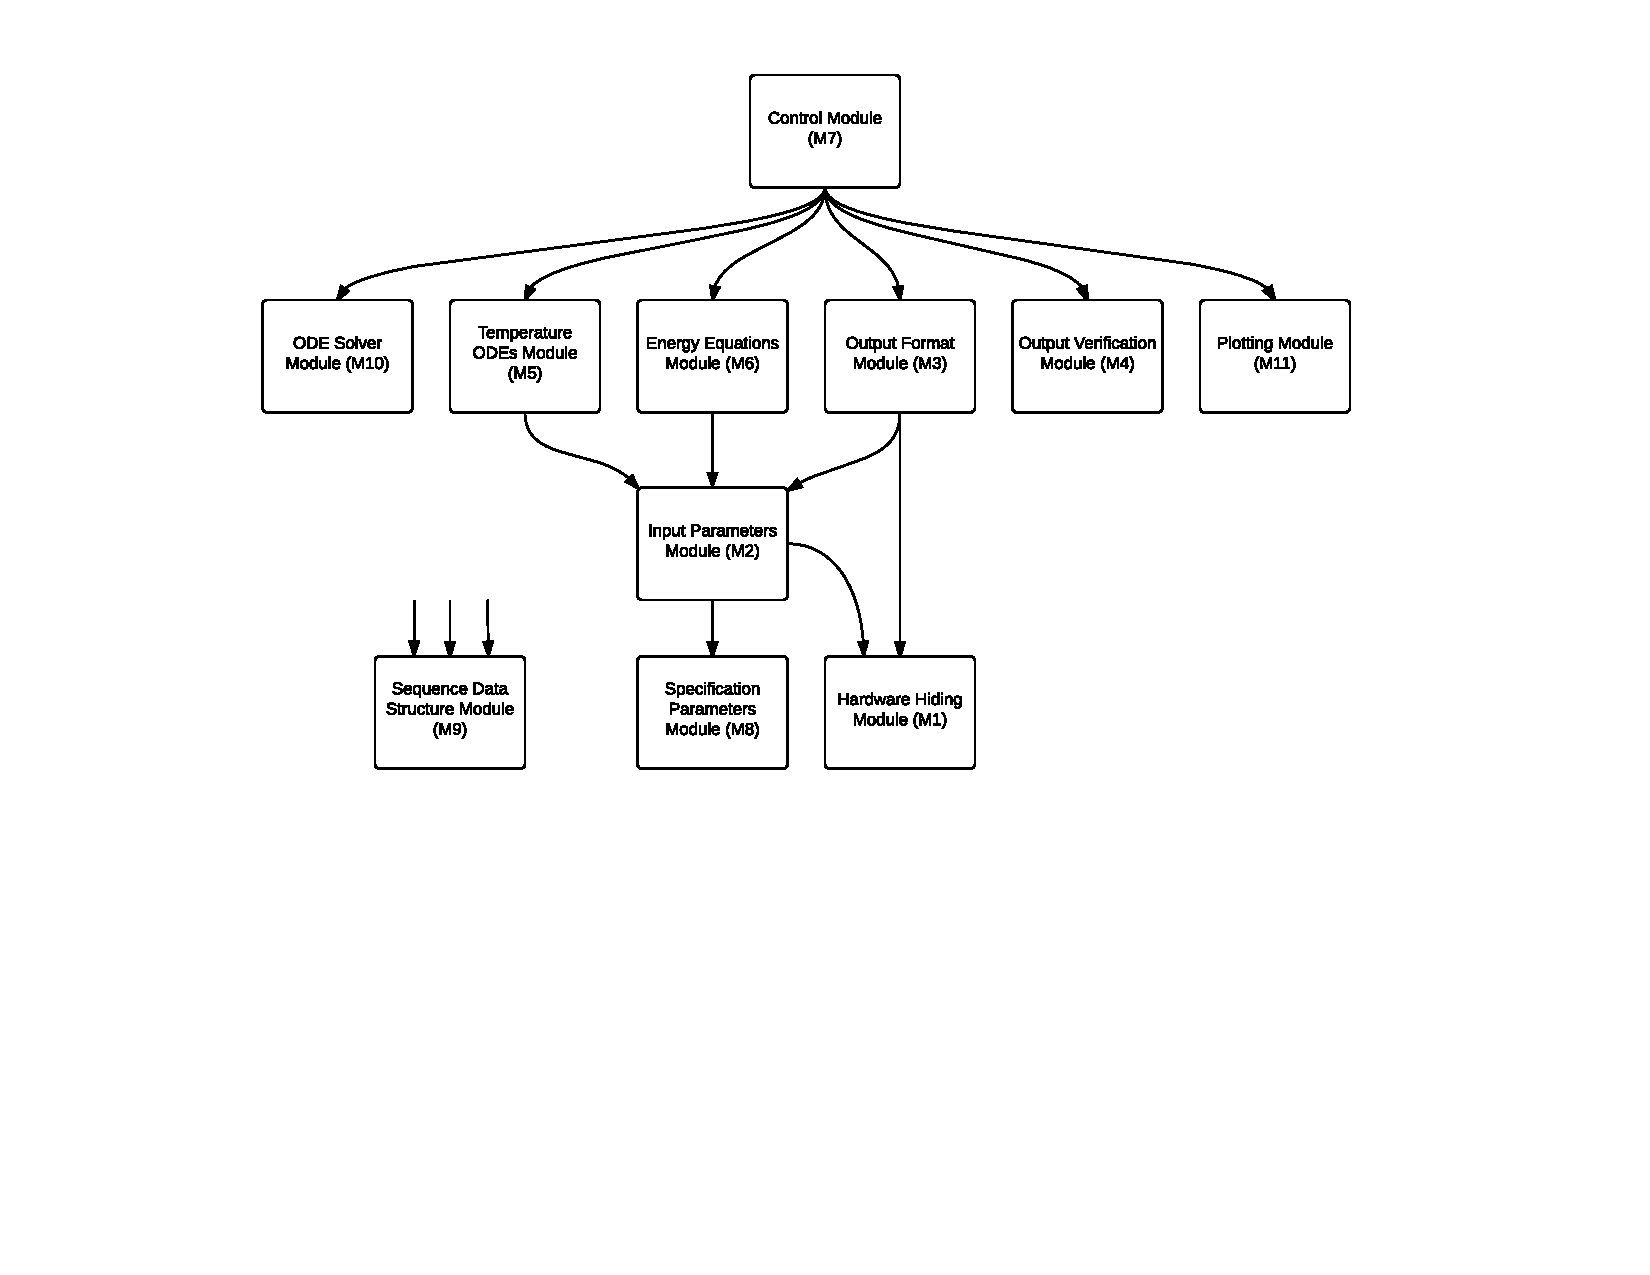
\includegraphics[scale=0.55]{../Figures/RevisedHierarchy.pdf}
\end{center}

\end{frame}

%%%%%%%%%%%%%%%%%%%%%%%%%%%%%%%%%%%%%%%%%%%%%%%%%%%%%%

\begin{frame}
\frametitle{Mesh Generator Example}
\vspace{-1cm}
\begin{figure}[H]
\includegraphics[scale=0.4, angle=0]{../Figures/ExampleMesh.pdf}
\end{figure}\end{frame}

%%%%%%%%%%%%%%%%%%%%%%%%%%%%%%%%%%%%%%%%%%%%%%%%%%%%%%

\begin{frame}
\frametitle{Mesh Generator Complex Circular Geometry}
\begin{figure}[H]
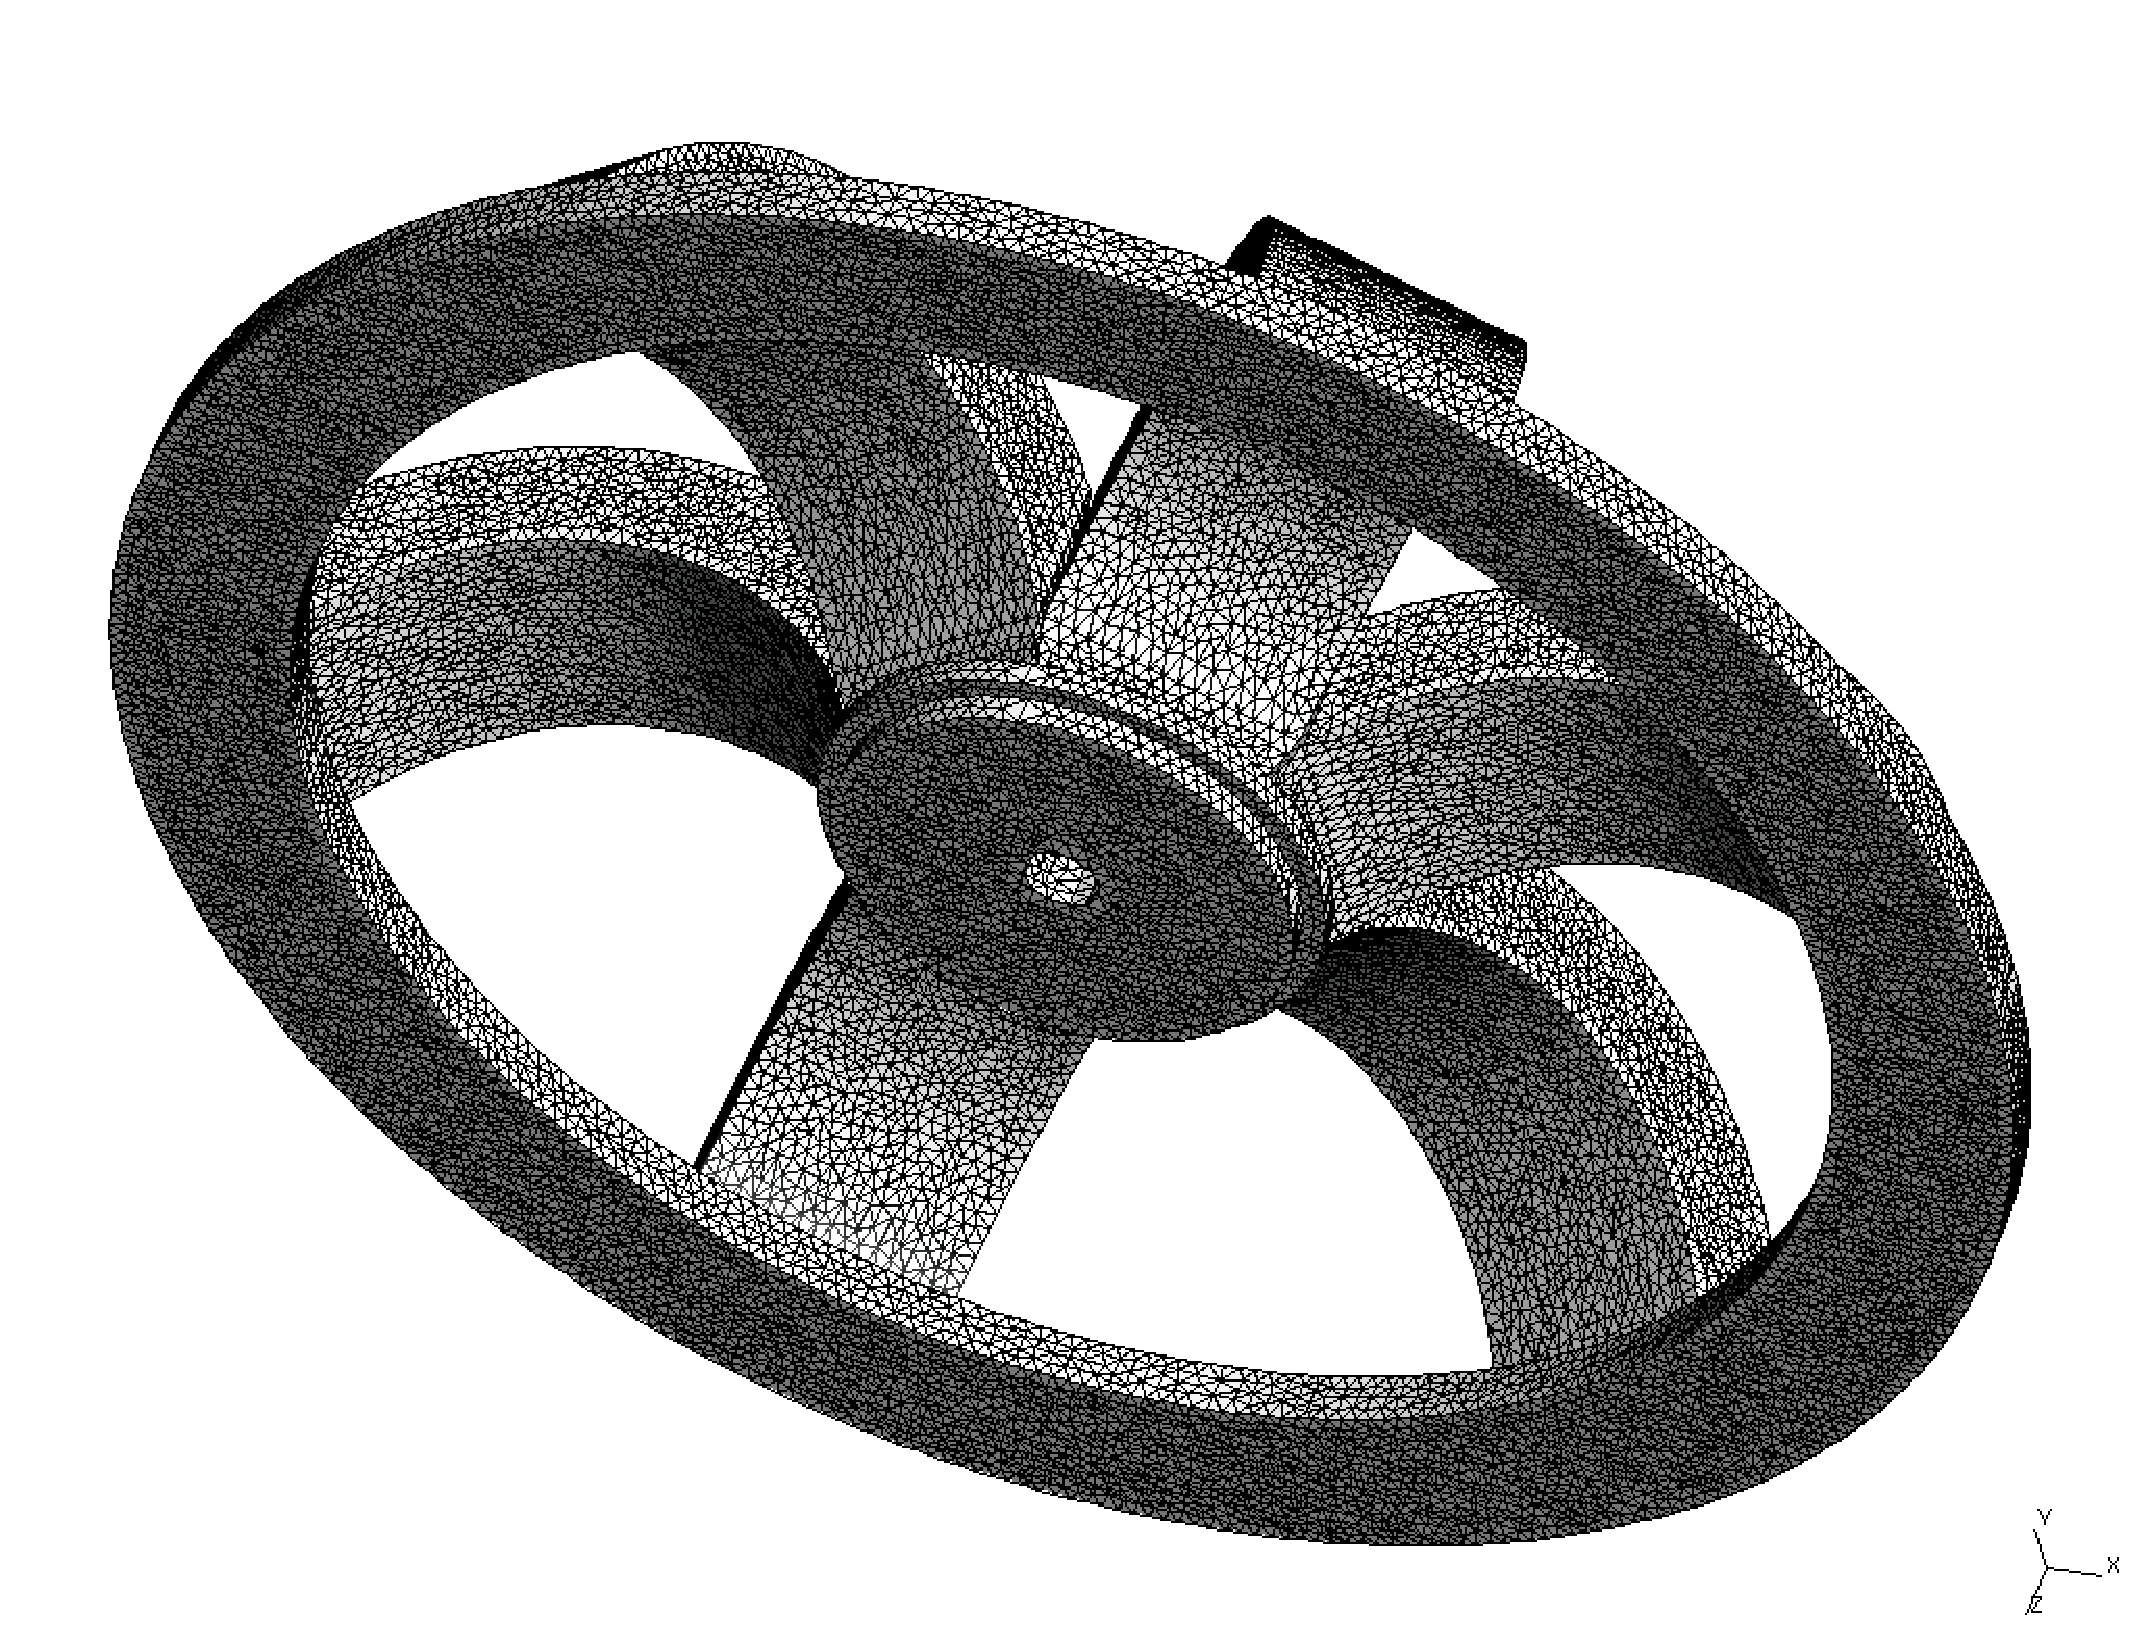
\includegraphics[scale=0.25]{../Figures/magnetron1.pdf}
\end{figure}\end{frame}

%%%%%%%%%%%%%%%%%%%%%%%%%%%%%%%%%%%%%%%%%%%%%%%%%%%%%%

\begin{frame}
\frametitle{Mesh Generator Example: Design Goals}
\begin{itemize}
\item Independent and flexible representation for each mesh entity
\item Complete separation of geometric data from the topology
\item The mesh generator should work with different coordinate systems
\item A flexible data structure to store sets of vertices, edges and triangles
\item Different mesh generation algorithms with a minimal amount of local changes
\end{itemize}
\end{frame}

%%%%%%%%%%%%%%%%%%%%%%%%%%%%%%%%%%%%%%%%%%%%%%%%%%%%%%

\begin{frame}
\frametitle{Example Mesh Gen Modular Decomposition}

%\vspace{-1.5cm}
% \begin{center}
% \includegraphics[width=0.5\textwidth]{DecompBySecretHierarchyExample.png}
% \end{center}

\href{https://gitlab.cas.mcmaster.ca/smiths/se2aa4_cs2me3/blob/master/Lectures/L14_ModuleDecompositionContinued/DecompBySecretHierarchyExample.png}{Link}

\end{frame}

%%%%%%%%%%%%%%%%%%%%%%%%%%%%%%%%%%%%%%%%%%%%%%%%%%%%%%

\begin{frame}
\frametitle{Another Mesh Generator Uses Hierarchy \cite{ElSheikhEtAl2004}}
\begin{figure}[H]
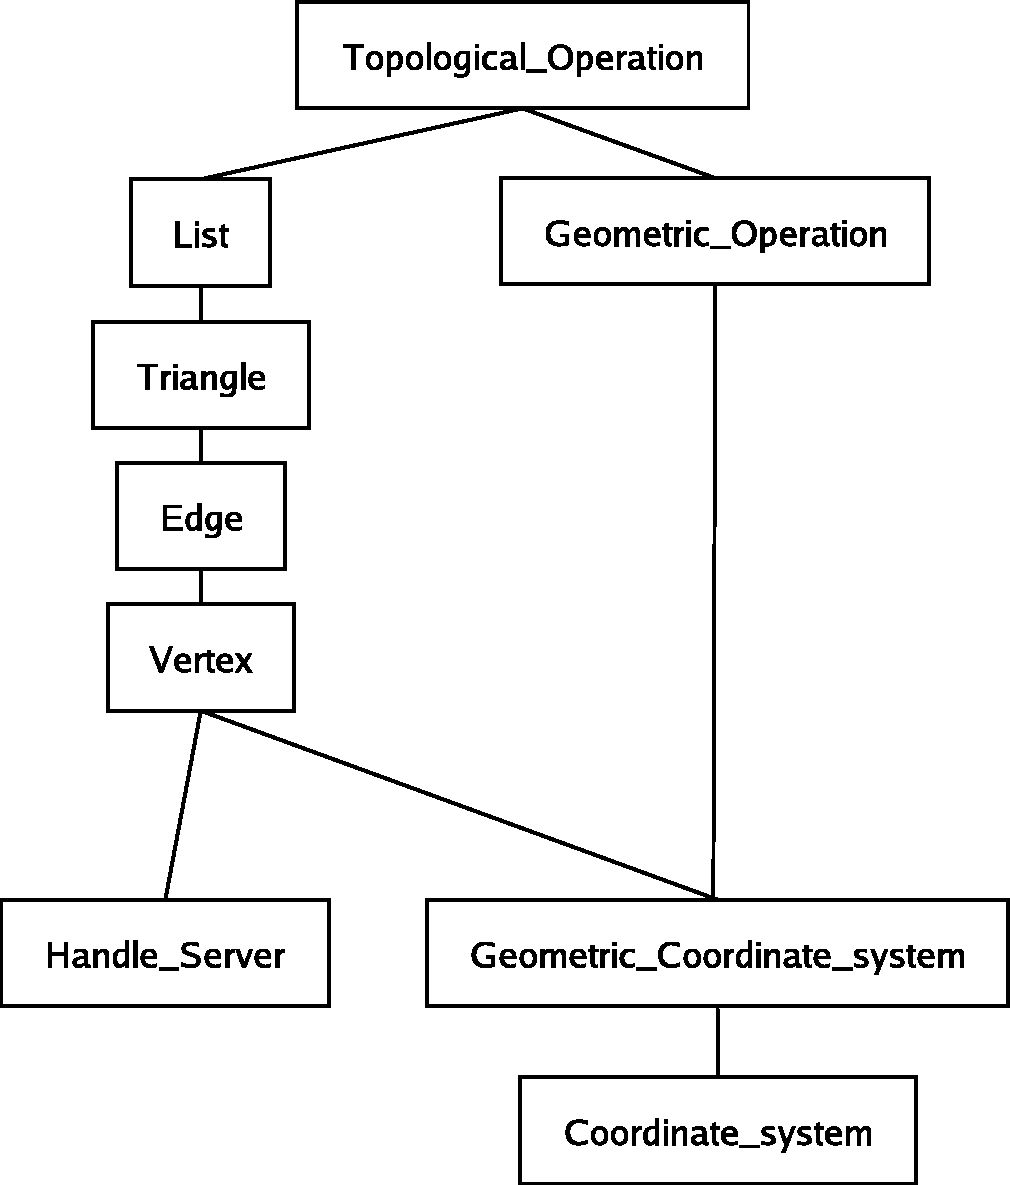
\includegraphics[scale=0.345]{../Figures/hierarchy_diagram.pdf}
\end{figure}
\end{frame}

%%%%%%%%%%%%%%%%%%%%%%%%%%%%%%%%%%%%%%%%%%%%%%%%%%%%%%

\begin{frame}
\frametitle{Module Testing}

\structure{Is it possible to begin testing before all of the modules have been
  implemented when there is a use relation between modules?}

\end{frame}

%%%%%%%%%%%%%%%%%%%%%%%%%%%%%%%%%%%%%%%%%%%%%%%%%%%%%%

\begin{frame}
\frametitle{Module Testing \cite{GhezziEtAl2003}}

\begin{itemize}

\item Scaffolding needed to create the environment in which the module should be
  tested
\item Stubs - a module used by the module under test
\item Driver - module activating the module under test
\end{itemize}

\end{frame}

%%%%%%%%%%%%%%%%%%%%%%%%%%%%%%%%%%%%%%%%%%%%%%%%%%%%%%

\begin{frame}
\frametitle{Testing a Functional Module \cite{GhezziEtAl2003}}

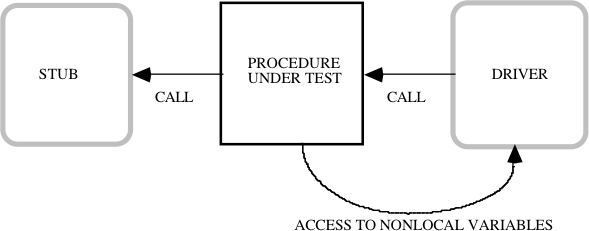
\includegraphics[scale=0.5]{../Figures/TestingAFunctModule.png}

\end{frame}

%%%%%%%%%%%%%%%%%%%%%%%%%%%%%%%%%%%%%%%%%%%%%%%%%%%%%%

\begin{frame}
\frametitle{Integration Testing}

\begin{itemize}
\item Big-bang approach
\begin{itemize}
\item First test individual modules in isolation
\item Then test integrated system
\end{itemize}
\item Incremental approach
\begin{itemize}
\item Modules are progressively integrated and tested
\item Can proceed both top-down and bottom-up according to the USES relation
\end{itemize}
\end{itemize}
\end{frame}

%%%%%%%%%%%%%%%%%%%%%%%%%%%%%%%%%%%%%%%%%%%%%%%%%%%%%%

\begin{frame}
\frametitle{Integration Testing and USES relation}

\begin{itemize}
\item If integration and test proceed bottom-up only need drivers
\item Otherwise if we proceed top-down only stubs are needed
\end{itemize}
\end{frame}

%%%%%%%%%%%%%%%%%%%%%%%%%%%%%%%%%%%%%%%%%%%%%%%%%%%%%%

\begin{frame}
\frametitle{Example \cite{GhezziEtAl2003}}

\begin{center}
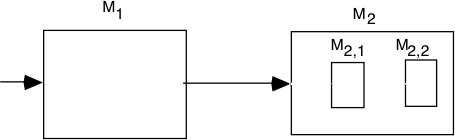
\includegraphics[scale=0.35]{../Figures/Example.png}
\end{center}

\begin{itemize}
\item $M_1$ USES $M_2$ and $M_2$ IS\_COMPOSED\_OF \{$M_{2,1}$, $M_{2,2}$\}
\item \structure{In what order would you test these modules?}
\end{itemize}
\end{frame}

%%%%%%%%%%%%%%%%%%%%%%%%%%%%%%%%%%%%%%%%%%%%%%%%%%%%%%

\begin{frame}
\frametitle{Example \cite{GhezziEtAl2003}}

\begin{center}
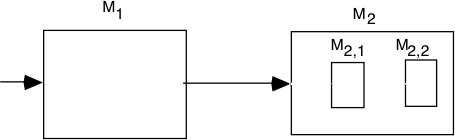
\includegraphics[scale=0.35]{../Figures/Example.png}
\end{center}

\begin{itemize}
\item $M_1$ USES $M_2$ and $M_2$ IS\_COMPOSED\_OF \{$M_{2,1}$, $M_{2,2}$\}
\item Case 1
\begin{itemize}
\item Test $M_1$ providing a stub for $M_2$ and a driver for $M_1$
\item Then provide an implementation for $M_{2,1}$ and a stub for $M_{2,2}$
\end{itemize}
\item Case 2
\begin{itemize}
\item Implement $M_{2,2}$ and test it by using a driver
\item Implement $M_{2,1}$ and test the combination of $M_{2,1}$ and $M_{2,2}$
  (i.e.\ $M_2$) by using a driver
\item Finally implement $M_1$ and test it with $M_2$ using a driver for $M_1$
\end{itemize}
\end{itemize}
\end{frame}

%%%%%%%%%%%%%%%%%%%%%%%%%%%%%%%%%%%%%%%%%%%%%%%%%%%%%%

\begin{frame}
\frametitle{Overview of MIS}
\begin{itemize}
\item See Hoffman and Strooper \cite{HoffmanAndStrooper1995}
\item The MIS precisely specifies the modules observable behaviour - what the module does
\item The MIS does not specify the internal design
\item The idea of an MIS is inspired by the principles of software engineering
\item Advantages
\begin{itemize}
\item Improves many software qualities
\item Programmers can work in parallel
\item Assumptions about how the code will be used are recorded
\item Test cases can be decided on early, and they benefit from a clear specification of the behaviour
\item A well designed and documented MIS is easier to read and understand than complex code
\item Can use the interface without understanding details
\end{itemize}
\end{itemize}
\end{frame}

%%%%%%%%%%%%%%%%%%%%%%%%%%%%%%%%%%%%%%%%%%%%%%%%%%%%%%

\begin{frame}
\frametitle{Overview of MIS}
\begin{itemize}
\item Options for specifying an MIS
\begin{itemize}
\item Trace specification
\item Pre and post conditions specification
\item Input/output specification
\item \structure{Before/after specification - module state machine}
\item Algebraic specification
\end{itemize}
\item Best to follow a template
\end{itemize}
\end{frame}

%%%%%%%%%%%%%%%%%%%%%%%%%%%%%%%%%%%%%%%%%%%%%%%%%%%%%%

\begin{frame}
\frametitle{MIS Template}

\begin{itemize}
\item Uses
\begin{itemize}
\item Imported constants, data types and access programs
\end{itemize}
\item Syntax
\begin{itemize}
\item Exported constants and types
\item Exported functions (access routine interface syntax)
\end{itemize}
\item Semantics
\begin{itemize}
\item State variables
\item State invariants
\item Assumptions
\item Access routine semantics
\item Local functions
\item Local types
\item Local constants
\item Considerations
\end{itemize}
\end{itemize}
\end{frame}

%%%%%%%%%%%%%%%%%%%%%%%%%%%%%%%%%%%%%%%%%%%%%%%%%%%%%%

\begin{frame}
\frametitle{MIS Uses Section}
\begin{itemize}
\item Specify imported constants
\item Specify imported types
\item Specify imported access programs
\item The specification of one module will often depend on using the interface specified by another module
\item When there are many modules the uses information is very useful for navigation of the documentation
\item Documents the use relation between modules
\end{itemize}
\end{frame}

%%%%%%%%%%%%%%%%%%%%%%%%%%%%%%%%%%%%%%%%%%%%%%%%%%%%%%

\begin{frame}
\frametitle{MIS Syntax Section}
\begin{itemize}
\item Specify exported constants
\item Specify exported types
\item Specify access routine names, the input and output parameter types and exceptions
\item Show access routines in tabular form
\begin{itemize}
\item Important design decisions are made at this point
\item The goal is to have the syntax match many implementation languages
\end{itemize}
\end{itemize}
\end{frame}

%%%%%%%%%%%%%%%%%%%%%%%%%%%%%%%%%%%%%%%%%%%%%%%%%%%%%%

\begin{frame}
\frametitle{Syntax of a Sequence Module}

\textbf{Exported Constants}\\
~\newline
MAX\_SIZE = 100\\

\end{frame}

%%%%%%%%%%%%%%%%%%%%%%%%%%%%%%%%%%%%%%%%%%%%%%%%%%%%%%

\begin{frame}
\frametitle{Syntax of a Sequence Module Continued}

\textbf{Exported Access Programs}\\
~\newline
\begin{tabular}{| l | l | l | l |}
\hline
\textbf{Routine name} & \textbf{In} & \textbf{Out} & \textbf{Exceptions}\\
\hline
seq\_init & ~ & ~ & ~\\
\hline
seq\_add & integer, integer & ~ & FULL, POS\\
\hline
seq\_del & integer & ~ & POS\\
\hline
seq\_setval & integer, integer & ~ & POS\\
\hline
seq\_getval & integer & integer & POS\\
\hline
seq\_size & ~ & integer & ~\\
\hline

\end{tabular}

\end{frame}

%%%%%%%%%%%%%%%%%%%%%%%%%%%%%%%%%%%%%%%%%%%%%%%%%%%%%%

\begin{frame}
\frametitle{MIS Semantics Section}

\begin{itemize}
\item State variables
\begin{itemize}
\item Give state variable(s) name and type
\item State variables define the state space
\item If a module has state then it will have ``memory''
\end{itemize}
\item State invariant
\begin{itemize}
\item A predicate on the state space that restricts the ``legal'' states of the module
\item After every access routine call, the state should satisfy the invariant
\item Cannot have a state invariant without state variables
\item Just stating the invariant does not ``enforce'' it, the access routine semantics need to maintain it
\item Useful for understandabilty, testing and for proof
\end{itemize}
\end{itemize}

\end{frame}

%%%%%%%%%%%%%%%%%%%%%%%%%%%%%%%%%%%%%%%%%%%%%%%%%%%%%%

\begin{frame}
\frametitle{Semantics Section Continued}

\begin{itemize}
\item Local functions, local types and local constants
\begin{itemize}
\item Declared for specification purposes only
\item Not available at run time
\item Helpful to make complex specifications easier to read
\end{itemize}
\item Considerations
\begin{itemize}
\item For information that does not fit elsewhere
\item Useful to tell the user if the module violates a quality criteria
\end{itemize}
\end{itemize}

\end{frame}

%%%%%%%%%%%%%%%%%%%%%%%%%%%%%%%%%%%%%%%%%%%%%%%%%%%%%%

\begin{frame}
\frametitle{Sequence MIS Semantics}

\textbf{State Variables}\\
$s$: sequence of integer
~\newline

\textbf{State Invariant}\\
$| s | \leq \mathrm{MAX\_SIZE}$
~\newline

\textbf{Assumptions}\\
seq\_init() is called before any other access program

\end{frame}

%%%%%%%%%%%%%%%%%%%%%%%%%%%%%%%%%%%%%%%%%%%%%%%%%%%%%%

\begin{frame}
\frametitle{Sequence MIS Semantics Continued}

\textbf{Access Routine Semantics}\\
~\newline
seq\_init():
\begin{itemize}
\item transition: $s := < >$
\item exception: none
\end{itemize}
~\newline
\noindent seq\_add($i, p$):
\begin{itemize}
\item transition: $s := s[0..i-1] || <p> || s[i..|s|-1]$
\item exception: $exc := (|s| = \mathrm{MAX\_SIZE} \Rightarrow  \mathrm{FULL} ~ | ~ i \notin [0..|s|] \Rightarrow
\mathrm{POS})$
\end{itemize}

\end{frame}

%%%%%%%%%%%%%%%%%%%%%%%%%%%%%%%%%%%%%%%%%%%%%%%%%%%%%%

\begin{frame}
\frametitle{Access Routine Semantics Continued}

\noindent seq\_del($i$):
\begin{itemize}
\item transition: $s := s[0..i-1] || s[i+1..|s|-1]$
\item exception:  $exc := (i \notin [0..|s|-1] \Rightarrow \mathrm{POS})$
\end{itemize}
~\newline
\noindent seq\_setval($i, p$):
\begin{itemize}
\item transition: $s[i] := p$
\item exception: $exc := (i \notin [0..|s|-1] \Rightarrow \mathrm{POS})$
\end{itemize}
~\newline
\noindent seq\_getval($i$):
\begin{itemize}
\item output: $out := s[i]$
\item exception: $exc := (i \notin [0..|s|-1] \Rightarrow \mathrm{POS})$
\end{itemize}

\end{frame}

%%%%%%%%%%%%%%%%%%%%%%%%%%%%%%%%%%%%%%%%%%%%%%%%%%%%%%

\begin{frame}
\frametitle{Access Routine Semantics Continued}

\noindent seq\_size():
\begin{itemize}
\item output: $out := | s |$
\item exception: none
\end{itemize}

\end{frame}

%%%%%%%%%%%%%%%%%%%%%%%%%%%%%%%%%%%%%%%%%%%%%%%%%%%%%%

\begin{frame}

\frametitle{Exception Signaling}

\begin{itemize}
\item Useful to think about exceptions in the design process
\item Will need to decide how exception signalling will be done
\begin{itemize}
\item A special return value, a special status parameter, a global variable
\item Invoking an exception procedure
\item Using built-in language constructs
\end{itemize}
\item Caused by errors made by programmers, not by users
\item Write code so that it avoid exceptions
\item Exceptions will be particularly useful during testing
\end{itemize}

\end{frame}

%%%%%%%%%%%%%%%%%%%%%%%%%%%%%%%%%%%%%%%%%%%%%%%%%%%%%%

\begin{frame}

\frametitle{Assumptions versus Exceptions}

\begin{itemize}
\item The assumptions section lists assumptions the module developer is permitted to make about the programmer's behaviour
\item Assumptions are expressed in prose
\item Use assumptions to simplify the MIS and to reduce the complexity of the final implementation
\item Interface design should provide the programmer with a means to check so that they can avoid exceptions
\item When an exceptions occurs no state transitions should take place, any output is {\it don't care}
\end{itemize}

\end{frame}

%%%%%%%%%%%%%%%%%%%%%%%%%%%%%%%%%%%%%%%%%%%%%%%%%%%%%%

\begin{frame}[allowframebreaks]
\frametitle{References}

\bibliography{../../ReferenceMaterial/References}

\end{frame}

%%%%%%%%%%%%%%%%%%%%%%%%%%%%%%%%%%%%%%%%%%%%%%%%%%%%%%

\end{document}